\section{Ablauf chemischer Reaktionen (Freiwilligkeit)}

\subsection{Enthalpie H / Reaktionsenthalpie $\Delta H_R$}
    Prinzip Energieminimum: Stoff will energiearmen Zustand erreichen!\\
    $\Delta H_R = H_{Produkte} - H_{Edukte} \quad [H] = \frac{kJ}{mol * K}$\\
    \vspace{-0.3cm}

\subsection{Entropie S / Reaktionsentropie $\Delta S$}
    Prinzip Energiemax: Stoffe eines Sys. mögl. grosse Unordnung an!\\
    \begin{tabular}{p{5.5cm}l}
        $\Delta S = \sum S^0_{Produkte} - \sum S^0_{Edukte}$ & $[\Delta S] = \frac{\color{red}J}{mol * K}$
    \end{tabular}\\
    $S^0$: Molare Standartentropie (1mol des Stoffs bei Std.Bedingungen)
\subsection{Freie Enthalpie $\Delta G$}
    Beschreibt Freiwilligkeit der Reaktion:\\
    \begin{tabular}{p{5.5cm}l}
        $\Delta G = \Delta H - T * \Delta S$ & $[\Delta G] = \frac{kJ}{mol}$
    \end{tabular}
    \begin{itemize}
        \item $\Delta G < 0:$ Exergon (freiwillige Reaktion)
        \item $\Delta G > 0:$ Endergon(unfreiwillige Reaktion)
    \end{itemize}

\subsection{Aktivierungsenergie/Reaktionsgeschw./Katalysatoren}
\begin{minipage}[t]{0.3\linewidth}
    \vspace*{0pt}
    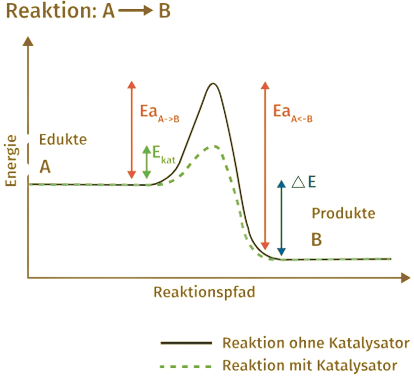
\includegraphics[width=\linewidth]{pictures/Katalysator.png}
\end{minipage}
\begin{minipage}[t]{0.7\linewidth}
\begin{itemize}
    \item RGT-Regel: $\Delta$ T = 10 $\rightarrow$ RG $\cdot$ 2
    \item Katalysator = Stoff nimmt an Reaktion teil, wird nicht verbraucht 
    \item Beschleunigt Reaktion: $E_{AKat} \ll E_{ANorm}$
    \item $\Delta$ G sowie $\Delta H_R$ bleiben gleich
    \item Selektiv (wirkt nicht mit allen Stoffen)
\end{itemize}
\end{minipage}
